\documentclass[11pt]{paper}

\input{insbox}
\usepackage[x11names]{xcolor}
\usepackage{lineno}

\usepackage{lib/utt-report-template}
\usepackage{lipsum}

\author{Tamas Spisak}
\date{2020}
\newcommand*\mytitle{\color{pniblue}\textbf{The Users' Manual}}

\newcommand*\mysubtitle{\color{pniblue} \textbf{A}nonymization with \\
\textbf{L}imesurvey integration and \\
\textbf{II}-factor \\
\textbf{A}uthentication for \\
\textbf{S}cientific research}
%\emph{ - dedicated for SFB289 -}

\newcommand*\myshorttitle{ALIIAS: The Users' Manual}
\newcommand*\version{1.0}
\title{\mytitle} % Max 144 chars

\schooltutor{}
\semester{}
\branch{}
\abstracttext{
Pseudonymization is a reversible de-identification process, in which personal data is converted to a \emph{pseudonym}, i.e. a unique identifier that can only be linked again to the personal data with certain restrictions (i.e. only by the single projects in SFB289). The main purpose of pseudonymization is to securely separate experimental from personal data. In clinical research, reversibility is required typically due to potential incidental findings.

A proper pseudonymization protocol can motivate the relaxation, to a certain degree, of data controllers’ legal obligations (if properly applied) \cite{pseudonym}, i.e. spare a significant amount of efforts put into data security and privacy, when storing, sharing and publishing experimental data and/or its derivatives.

Issues of privacy protection are part of a rapidly changing 'landscape' shaped by ongoing digitalization efforts (in general and specifically in medical research) and by the recent developments in the corresponding regulations (most importantly the GDPR \cite{gdpr}). Recent developments in  this filed render some of the 'traditional' pseudonymization methods, which have been typically used so far in medical research (e.g. the frequently used sequential numbering of participants), increasingly “outdated”, with significant safety concerns (e.g. vulnerability stemming from storing and regularly updating a document linking the personal data to the IDs, or possibility of adversarial re-identification based on the order of data in the pseudonymized dataset).

Here we propose a software tool, called ALIIAS, which implements a de-centralized, encryption-based deterministic pseudonymization technique to transform personal data to a pseudonym.
The 'full version' of the pseudonym (long ID) allows for complete re-identification (given a dedicated secret digital key, owned by the 'pseudonymization entity', i.e. the individual research site). The software also provides a 'human-readable' (9 characters) and scannable (barcode)  short ID, which is easy to link to the long ID and is compatible with most experimental procedures.

PseudoID is equipped with integration to LimeSurvey \cite{limesurvey}, an open-source web application for digital, web-accessible surveys and questionnaires.

\par\noindent\rule{\textwidth\color{pniblue}}{0.4pt}

\textbf{Highlights: }
\begin{itemize}
    \item pseudonymization happens as a first step of the experiment, so that all succeeding steps already work with anonymized data;
    \item pseudonyms are deterministic, i.e. reproducible in case of multiple measurements;
    \item pseudonyms are guaranteed to be unique, even for multi-center experiments;
    \item pseudonymization can be performed at multiple computers/sites simultaneously
    \item pseudonymization happens after a two-factor authentication, and requires a hardware key;
    \item no central administration of the link between pseudonym and personal data is needed
    \item the "pseudonymization secret" is restricted to a single point: to the USB hardware keys.
\end{itemize}





}

\setcounter{tocdepth}{4}

\begin{document}

    %\setlength{\parskip}{0mm}
    %\linenumbers
    \titlespacing*{\section}
    {0pt}{1cm plus 2cm minus 0cm}{0.2cm plus 2cm}
    \titlespacing*{\subsection}
    {0pt}{0.2cm plus 2cm minus 0cm}{0.2cm plus 2cm}

    \frontpage
    
    \begin{small}
    \setlength{\parskip}{1mm}
    
    \pagenumbering{arabic}
    \setcounter{page}{2}
    
    \tableofcontents
    \addtocontents{toc}{~\hfill\textbf{\color{pniblue}Page}\par}
    \thispagestyle{fancy}
    \pagebreak
    
    \end{small}
    \begin{large}
    
    \section{Overview of the pseudonymization procedure}
\label{section:overview}
ALIIAS has a number of assumption about the underlying experimental procedures. These assumptions were defined so that they are easy to fit to the majority of medical research experiments. The pseudonymization workflow of SFB289 is illustrated on Fig. \ref{fig:flowchart} and includes the following steps.

\begin{figure}[H]
\centering
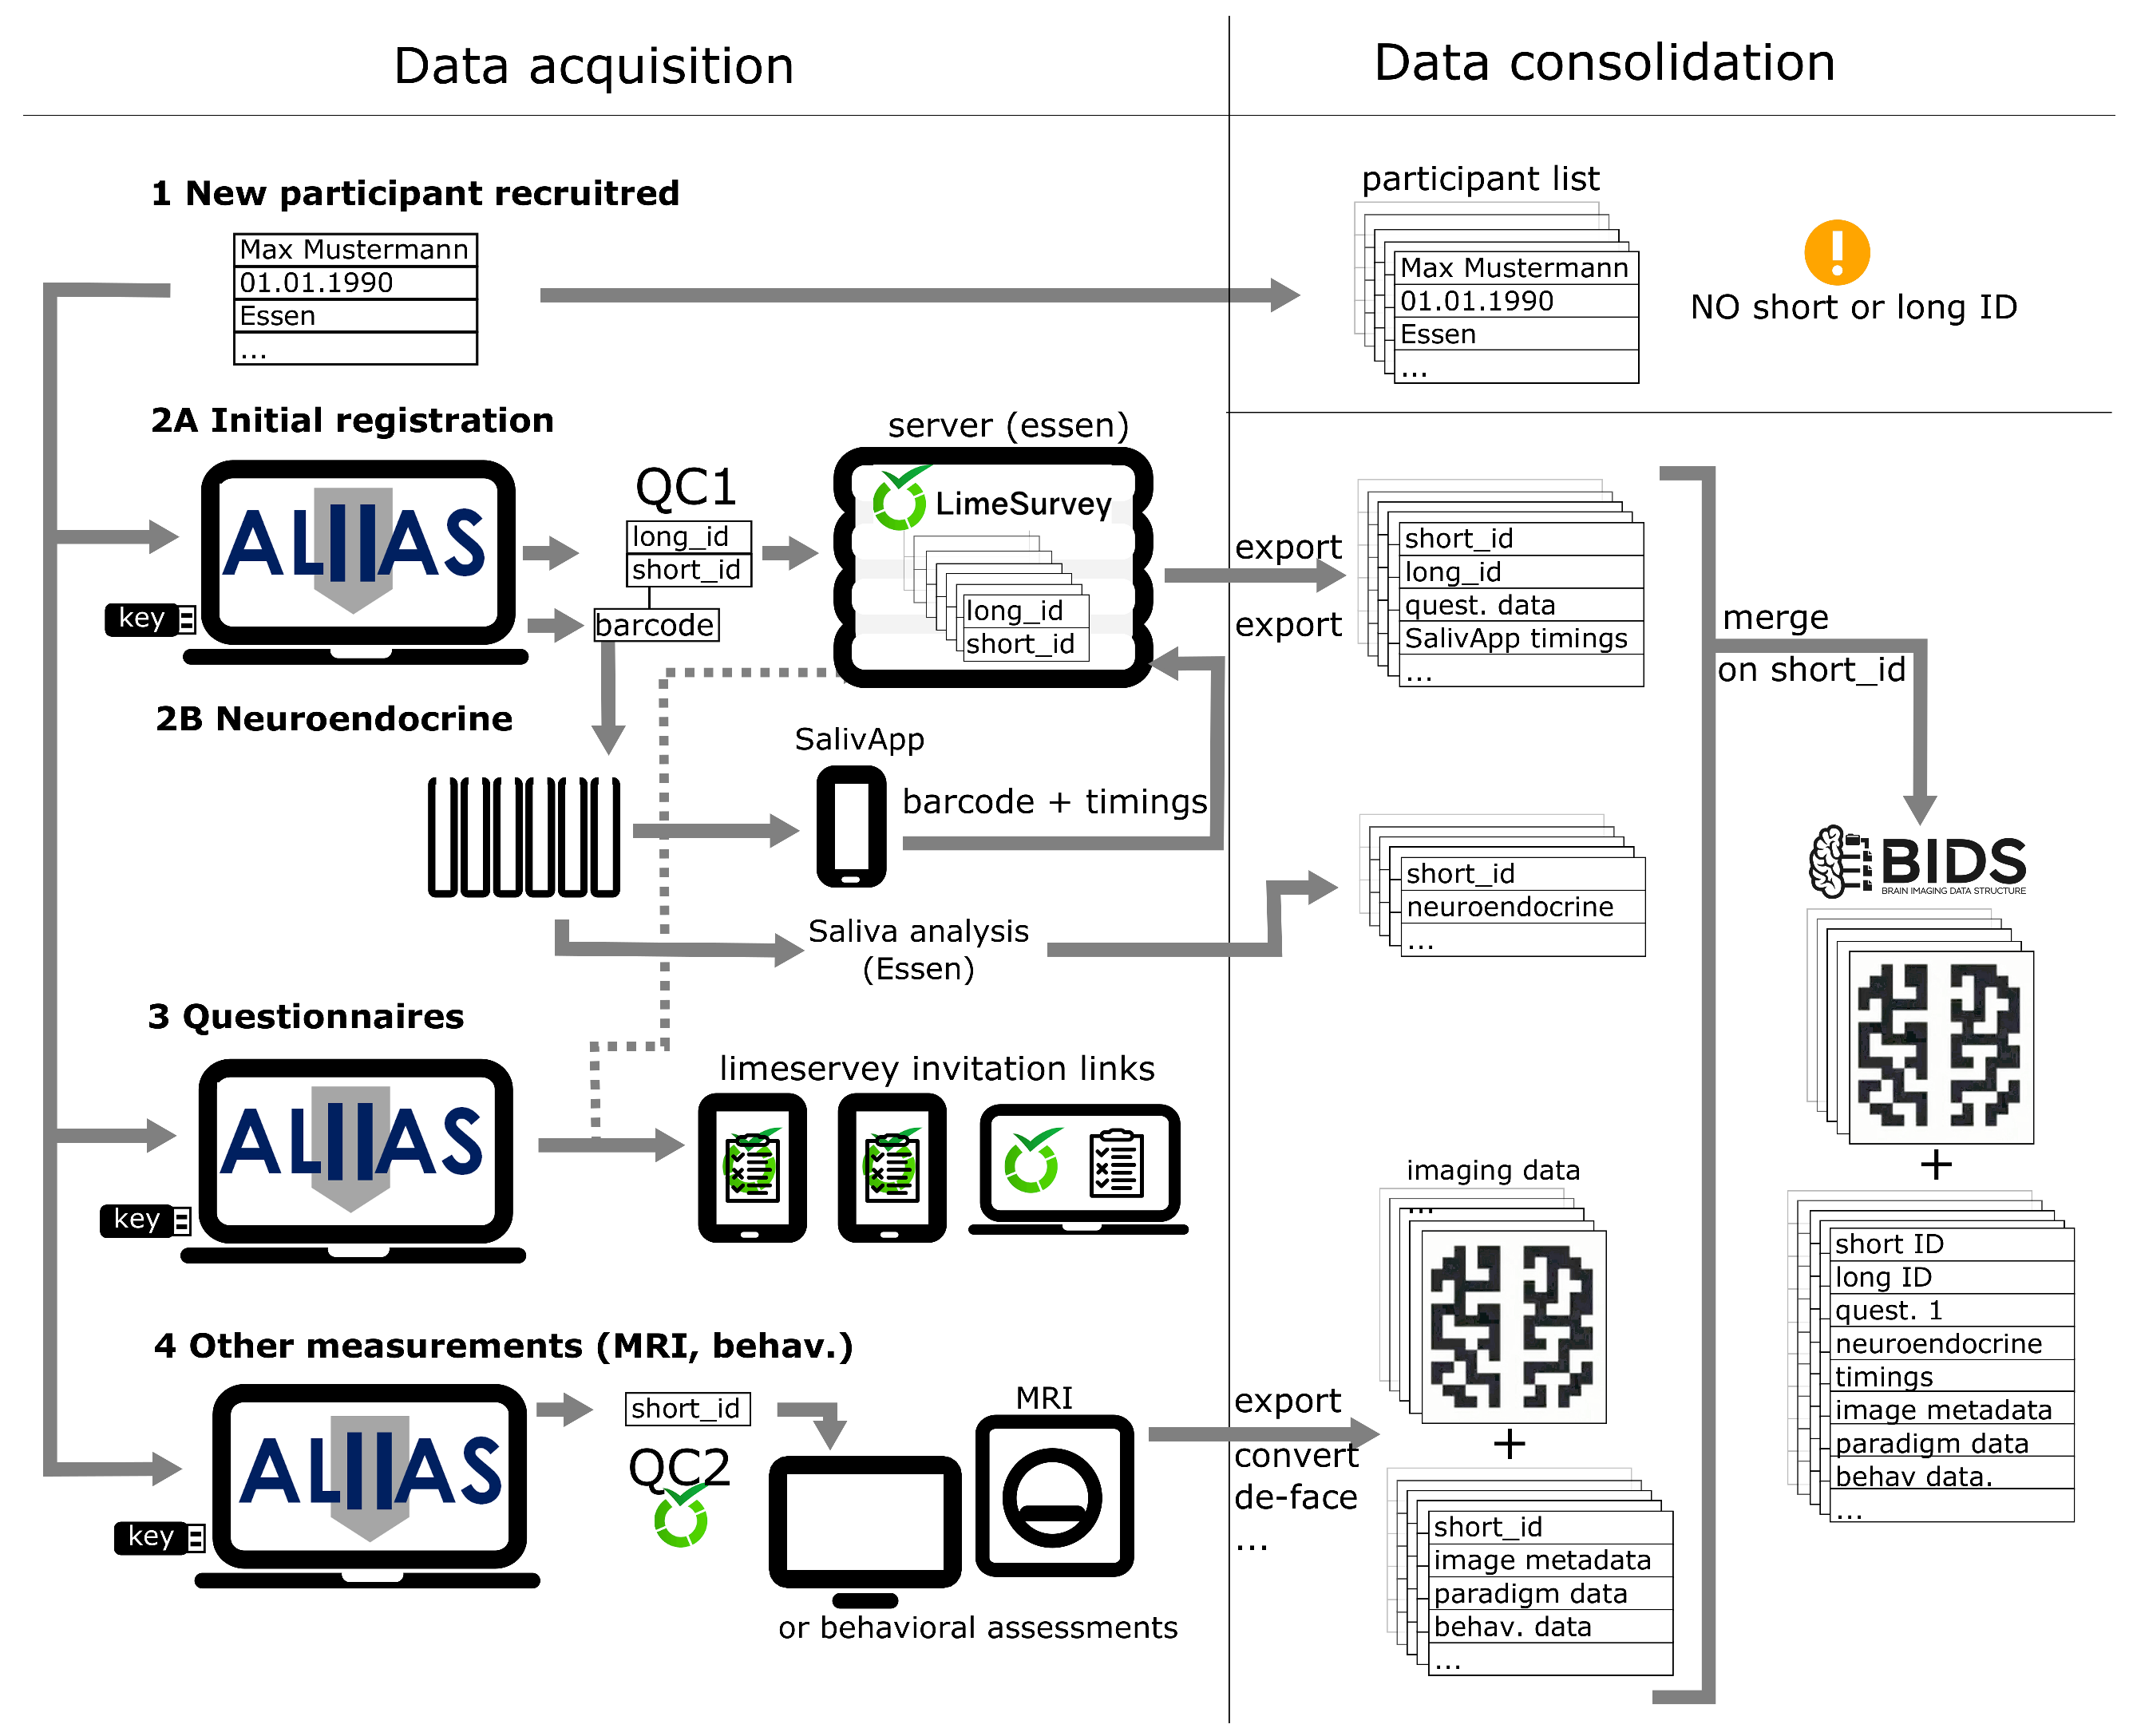
\includegraphics[width=1.0\textwidth]{docs/fig/overview_v3.eps}
\caption{The pseudonymization workflow of SFB289}
\label{fig:flowchart}
\end{figure}

\InsertBoxR{1}{
\small\setlength\fboxsep{5pt}\setlength\fboxrule{1pt}
\fcolorbox{pniblue}{pniblue!5}{\begin{minipage}{0.5\textwidth}
Important Note: the pseudonyms must never be stored in the participant list!
\end{minipage}}
}[1]

\par\noindent\rule{\textwidth\color{pniblue}}{0.4pt}
\textbf{1. Participant recruitment:}
\addcontentsline{toc}{subsubsection}{Participant recruitment}
When a new participant is recruited, his/her personal data and contact details (e.g. address, phone number, e-mail) is recorded on-site (or e.g. during a telephone interview). These data is typically saved into a "participant list" (often an excel table, its maintenance is the responsibility of the single projects, see Fig. \ref{fig:flowchart}). While this participant list itself is also to be protected, ALIIAS is not reliable for the protection of this data. In fact, the main goal of ALIIAS is to make it impossible to link this data to the experimental datasets (unless owning the pseudonymization secret, i.e. the hardware key).
%%\par\noindent\rule{\textwidth\color{pniblue}}{0.4pt}
%\InsertBoxR{-1}{
%\small\setlength\fboxsep{5pt}\setlength\fboxrule{1pt}
%\fcolorbox{pniblue}{pniblue!5}{\begin{minipage}{0.45\textwidth}
%Importantly, even though the web browser is used as a user interface for the software %(thus it looks like a webpage), personal data always stays on the local computer hosting %the software and hardware key.
%\end{minipage}}
%}[1]


\par\noindent\rule{\textwidth\color{pniblue}}{0.4pt}
\addcontentsline{toc}{subsubsection}{Initial registration}
\textbf{2A. Initial registration:} The dedicated hardware key (provided by Z03) is connected to an experimental computer (with ALIIAS already installed) via the USB port. As a next step, the researcher enters the LimeSurvey login credentials in ALIIAS and the provides the following personal data of the participant on the browser interface of ALIIAS (depicted on the left of Fig. \ref{fig:screenshots}):
\begin{itemize}
    \item first name
    \item last name
    \item date of birth
    \item place of birth
    \item mother's maiden name
\end{itemize}

Importantly, even though the web browser is used as a user interface for the software (thus it looks like a webpage), \textbf{personal data always stays on the local computer}, which hosts the software and hardware key.


\begin{figure}[H]
%\centering
\subfigure{\includegraphics[width=.45\textwidth]{docs/fig/03_filled.PNG}}
\hfill
\subfigure{\includegraphics[width=.45\textwidth]{docs/fig/05_pseudonym.PNG}}
\caption{The browser-based user interface of ALIIAS.}
\label{fig:screenshots}
\end{figure}

ALIIAS reads the "pseudonymization secret" from the hardware key and uses it to generate pseudonym. After the user confirms that the data is correct, the software outputs the long and short-version of the pseudonym (on the right of Fig. \ref{fig:screenshots}). Both the long and short IDs are unique for the whole CRC. De-identification is only possible with the long-id. During the initial registration, ALIIAS automatically connects to the LimeSurvey server hosted at the University Duisburg-Essen and registers the participant's long and short IDs to any of the surveys belonging to the single project. Additionally, ALIIAS converts the short ID into a barcode (see step 5) for labelling assessment tools belonging to the participant.

\par\noindent\rule{\textwidth\color{pniblue}}{0.4pt} 
\addcontentsline{toc}{subsubsection}{Compatibility with neuroendocrine and genetic assessments}
\textbf{2B. Compatibility with neuroendocrine and genetic assessment and Biobank:} Upon the initial registration, ALIIAS generates a set of barcodes, encoding the short ID. These will be printed by the barcode printers provided by the central projects and used to label the saliva sampling kit (+ genetics) for the given participant (refer to the corresponding SOP of Z02). These barcode labels will be scanned by the participant, using the dedicated smartphone application of SFB289 (SalivApp), directly after during sample collection (for precise timing). The ShortID encoded in the barcode is obtained in Z02 to link saliva sample results with sample timings, genetics and BioBank-IDs.

\par\noindent\rule{\textwidth\color{pniblue}}{0.4pt}
\addcontentsline{toc}{subsubsection}{Questionnaires}
\textbf{3. Questionnaires:}
 In SFB289, questionnaire data will be collected with LimeSurvey. After the participant has been assigned to a survey, ALIIAS provides an individualized invitation link, which can be opened in another browser tab or e-mailed to the participant. Questionnaires can be filled in on any computer (or tablet), with internet connection. 
 If the initial registration and the assignment of the participant to a given questionnaire take place in different time points (e.g repeated measures), ALIIAS can be used again and again to obtain the (permanent) short ID of the participant, given his/her personal data (either from the local 'participant list', see step 1., or as provided by the participant.
 Multiple assessment points (repeated measures) are handled as separate surveys in LimeSurvey (refer to section \ref{section:ls_setup} for more details).
 
 \par\noindent\rule{\textwidth\color{pniblue}}{0.4pt}
 \addcontentsline{toc}{subsubsection}{Other measurements}
 \textbf{4. Other measurements (MRI, behavior):}
 For other measurements, ALIIAS can be used repeatedly to obtain the shortID of the participant (given the hardware key). The short ID can than be used in the dedicated experimental system (e.g. the MRI console) as the identifier ("name") of the participant, so that it gets exported together with the experimental data. In case of repeated measurements, ALIIAS is simply used multiple times to obtain the short ID. Single projects can add arbitrary "experimental tags" to the short ID (e.g. append '-w2' for week 2) or use the built in features of the given experimental equipment (e.g. separate 'program cards' on the MRI console) to distinguish between measurements.

\par\noindent\rule{\textwidth\color{pniblue}}{0.4pt}
\addcontentsline{toc}{subsubsection}{Data Consolidation and re-identification}
\textbf{Data Consolidation and re-identification:} The experimental data (either exported form the LimeSurvey database, or via the dedicated experimental systems) - if required - will be subject of further anonymization (e.g. de-facing of structural MRI images) The central scientific project will provide recommendations and share software tools for these tasks. Merging of experimental data from different sources or different assessment points is based on the short ID. The LimeSurvey database provides the link between the short and long IDs. The latter can be used for re-identification, e.g. in case of incidental findings by the owners of the hardware key.
    %\par\noindent\rule{\textwidth\color{pniblue}}{0.4pt}
\section{Example use-cases}
\par\noindent\rule{\textwidth\color{pniblue}}{0.4pt}
\textbf{1. Initial registration only (one-session use-case):}
If only questionnaires are collected or all assessments are done in one session, the initial registration with PseudoID might already be sufficient. In this case, the new participant must be assigned to all necessary surveys in LimeSurvey and must be invited to all, during the initial registration. The short ID generated during the initial registration can be used for any additional subsequent assessments, directly following the initial registration.

\par\noindent\rule{\textwidth\color{pniblue}}{0.4pt}
\textbf{2. "Batched" initial registration of many subjects (multi-session use-case):}
With the proposed pseudonymization procedure, the researcher has the opportunity to "batch" initial registrations, i.e. perform the initial registration of many participants in one longer session, based on the personal data previously collected (e.g. during phone interview). The assignment of the participants to specific surveys and the actual experiments (MRI, behavior) can take place at a later time point. In this case, PseudoID can be used multiple times to repeatedly obtain the pseudonym for a given participant. In this case, a database query is performed that allows for checking for typos in the personal data and ensure that the proper short ID is obtained.

\par\noindent\rule{\textwidth\color{pniblue}}{0.4pt}
\textbf{3. Repeated assessments (multi-session + repeated measures use-case):}
Use-case 2 is easy to adapt to repeated assessments (e.g. before and after treatment).
For convenience, PseudoID provides a pre-defined subset of "experimental tags" (e.g. baseline, week1, week2, etc) which is appended to the short ID.

\par\noindent\rule{\textwidth\color{pniblue}}{0.4pt}
\textbf{4. Simultaneous assessment of many subjects (parallel-sessions use-case):}
PseudoID can be run on multiple computers simultaneously without any further notice. The reproducibility and uniqueness of pseudonyms and the consistency of the LimeSurvey database are still guaranteed.

\par\noindent\rule{\textwidth\color{pniblue}}{0.4pt}
\textbf{5. Computer failure during experiment:}
If the experiment has to be restarted, PseudoID can be repeatedly used to obtain the short ID. In the case of failure of the computer on which PseudoID runs, a backup computer can be used to obtain the short ID (even if the initial registration and other pseudonymization sessions were not performed on that computer).

\par\noindent\rule{\textwidth\color{pniblue}}{0.4pt}
\textbf{6. Incidental finding:} In case of incidental finding, the LimeSurvey database will be used to link the long ID to the short ID and re-identification is performed by PseudoID (on any computer), given the long ID and the pseudonymization secret stored on the hardware key. 
    \section{SOP: Installation}
\label{section:sop_installation}
ALIIAS can be installed on Windows computers. The installation procedure requires administrator privileges (i.e authorization from the IT department, in case of centrally-administered computers; for each installation individually).

\begin{itemize}
    \item Navigate to the \path{ALIIAS/latest} folder in the SFB289-cloud to access the latest version of ALIIAS.
    
    SFB289-cloud: \href{https://uni-duisburg-essen.sciebo.de/s/yYzEg59bvl8focL}{\color{pniblue}{https://uni-duisburg-essen.sciebo.de/s/yYzEg59bvl8focL}}
    
    (password already disclosed in email)
    
    \item Download and extract the zip archive (ALIIAS\_v*.zip) to an arbitrary folder. This will result in the following files\footnote{If you can not see the file extensions, you should activate them under "View" in the explorer}: 
    \begin{itemize}
        \item \path{start_ALIIAS.exe}
        \item \path{ALIIAS.txt}
        \item \path{handler.txt}
        \item \path{settings.conf} 
        \item \path{opensc-pkcs11.dll}
    \end{itemize}
    \item If you have administrator privileges on the computer, simply double-click the file called \path{start_ALIIAS.exe} to start the software.
    
    Refer to the instructions below if you are working on a centrally administered computer.
\end{itemize} 
\par\noindent\rule{\textwidth\color{pniblue}}{0.4pt}

\subsection*{Installation on centrally-administered computers}

Please contact the IT department (via phone call or helpdesk ticket) and ask for privileges for running the software. Explain the IT department what the software exactly does: "ALIIAS is a research software for SFB289. Technical details: it is a 'flask' application deployed as a standalone exe file. It depends on the OpenSC library, for handling harwarekeys. The dll for this dependency is shipped with the installation for convenience. The path to the dll can be set in the file \path{settings.conf} if needed. ALIIAS on startup reads the dependency's .dll file and two configuration files (from the same folder the executable is in) and runs a webserver on the localhost (Port 5000)".

In addition, you can provide the following steps to the IT-administrator (a solution working at the University Hospital Essen).

\begin{enumerate}
    
    \item The administrator from the IT department should move the \path{start_ALIIAS.exe}, \path{handler.txt}, \path{settings.conf} and \path{opensc-pkcs11.dll} files to a directory, from which the \path{.exe} can be executed. Caution: They have to be in the SAME folder. 
    
    \item The \path{ALIIAS.txt} file should be moved to a location that can be accessed by the user, for example the desktop. The file should then be opened with a text editor, to change the current path to the path where the \path{.exe} was moved to.
    \label{item:admin}
    
    \item For example: after installation, the contents of \path{ALIIAS.txt} end like this: \\ \path{.\ALIIAS.exe}. \\ This should be changed to the NEW path of the \path{start_ALIIAS.exe}
    
    \item When this has been changed correctly, the file name of \path{ALIIAS.txt} has to be changed to \path{start_ALIIAS.bat} (you can ignore the warning)
    
    \item If everything worked out properly, a double-click on \path{start_ALIIAS.bat} should start ALIIAS in a new browser window.
\end{enumerate} 

\subsection*{Installation on MacOS}
Installation is analogous to the Windows installation, except that some file extensions will be different (\path{.so} instead of \path{.dll}, no extension instead of \path{.exe}).

\vspace{2mm}

\small\setlength\fboxsep{5pt}\setlength\fboxrule{1pt}
\fcolorbox{pniblue}{pniblue!5}{\begin{minipage}{0.9\textwidth}
WARNING: ALIIAS v1.0 was not exhaustively tested on MacOS.
\end{minipage}}

\small\setlength\fboxsep{5pt}\setlength\fboxrule{1pt}
\fcolorbox{pniblue}{pniblue!5}{\begin{minipage}{0.9\textwidth}
On MacOS, ALIIAS v1.0 takes some more seconds to start up. Upon exit, the ALIIAS command line window (black character terminal) remains open and must be closed manually.
\end{minipage}}


    \pagebreak
\section{SOP: Setting up LimeSurvey for compatibility with ALIIAS}
\label{section:ls_setup}

\subsection*{General information about LimeSurvey}

\begin{wrapfigure}{r}{0.5\textwidth}
\centering
\includegraphics{docs/fig/ls_conventions.png}
\caption{LimeSurvey's terminology.}
\label{fig:ls_conventions}
\end{wrapfigure}

LimeSurvey is a free and open source on-line statistical survey web app (www.limesurvey.org).
In LimeSurvey, a series of questions, which are supposed to be filled-in by the same person, in one session; is called a \emph{survey} (Fig. \ref{fig:ls_conventions}).
In SFB289, multiple assessment points or visits within one study will be represented by multiple surveys.
A survey typically consists of many questionnaires (“Fragebögen”), which are called “question groups” in LimeSurvey.
LimeSurvey provides the opportunity to limit survey access to those participants only, who were previously registered to a so-called participant table (“Teilnehmertabelle”) of the survey by the researcher. In SFB289, ALIIAS will generate pseudonyms for participants and – after the proper setup of LS – automatically register the participants (with their pseudonyms) to the surveys specified by the researcher. Moreover, the link (URL) for these surveys can also be obtained from ALIIAS. The following steps explain how to set up LimeSurvey for compatibility with ALIIAS.

\par\noindent\rule{\textwidth\color{pniblue}}{0.4pt}
\subsection*{Step 1. Log in to LimeSurvey.}
The URL for the CRC-wise LimeSurvey server is:

\hyperref[https://sfb289.survey.uni-due.de/index.php/admin/authentication/sa/login]{https://sfb289.survey.uni-due.de/index.php/admin/authentication/sa/login}

Log in credentials will be sent out individually. 

\par\noindent\rule{\textwidth\color{pniblue}}{0.4pt}
\subsection*{ Step 2. Creating a new SFB289-survey.}
The single projects in SFB289 can have multiple surveys, e.g. one survey for each measurement time point (“visit”). For studies in which the researcher or study doctor is also supposed to fill in a questionnaire/checklist, multiple surveys for each visit should be used (see step 2.3).

When creating a new survey, we have access to the standard questionnaire battery of SFB289. To include it, new surveys must be created by copying the survey \\ “SFB289\_standard\_questionnaire\_battery” as many times as needed. 

\par\noindent\rule{\textwidth\color{pniblue}}{0.4pt}
\subsubsection*{2.1. Choose “Kopieren Sie eine Umfrage” on the home screen.}
\begin{figure}[H]
\includegraphics[width=0.5\textwidth]{docs/fig/ls_sop2.1.png}
\end{figure}

\par\noindent\rule{\textwidth\color{pniblue}}{0.4pt}
\subsubsection*{2.2 Select the “Kopieren” tab, select the survey called “SFB289\_standard\_questionnaire\_battery” for copy. }
\begin{figure}[H]
\includegraphics[width=1.0\textwidth]{docs/fig/ls_sop2.2.png}
\end{figure}

\par\noindent\rule{\textwidth\color{pniblue}}{0.4pt}
\subsubsection*{2.3 Give the new survey a name according to the following rule:} <project>\_<study>\_<measurement>\_<target>

\subsubsection*{Explanation:}
\begin{itemize}
    \item <project>: the name of the single project within the SFB. Must consist of an uppercase “A” letter and a two-digit number (A01, A02, …, A16). Our pseudonymization software (called ALIIAS) uses this part of the name to restrict visibility of surveys.
    \item <study>: an arbitrary identifier to distinguish studies if multiple studies are performed within one project. (e.g. study1, follow-up, etc.). Can be omitted if only one study is performed. 
    \item <measurement>: a name for measurement time point (e.g. baseline, visit1, day1, pre, post, etc). Can be omitted if the study involves only one measurement time point.
    \item <target>: the “role” of the person who fills in the survey. (e.g. participant, doctor, interviewer, etc). Can be omitted if all surveys are filled in by the participants.
\end{itemize}

Separator must be underscore (\_). Refer to Table \ref{tab:example_names} for some valid examples for survey names. Click on “Umfrage kopieren” to create the new survey.
\begin{table}[h]
 \caption{Example survey names, compatible with ALIIAS.}
  \centering
  \begin{tabular}{ll}
    \toprule
    Survey names      & Explanation      \\
    \midrule
    \midrule
    A01            & a hypothetical A01 project consisting of a single survey only                 \\
    \midrule
    A02\_visit1           & a hypothetical A02 project, having two visits \\
    A02\_visit2      & \\
    \midrule
    A03\_study1           & a hypothetical A03 project,               \\
    A03\_study2\_visit1          &  having two studies and two visits in the second study              \\
    A03\_study1\_visit2           &                \\
    \midrule
    A04\_visit1\_participant      &   a hypothetical A04 project,             \\
    A04\_visit1\_doctor           &   having separate surveys for the participant and the study doctor           \\
    \bottomrule
  \end{tabular}
  \label{tab:example_names}
\end{table}

\par\noindent\rule{\textwidth\color{pniblue}}{0.4pt}
\subsection*{Step 3. Edit the new survey as needed. }

\begin{wrapfigure}{r}{0.5\textwidth}
\centering
\includegraphics{docs/fig/ls_sop3.png}
\end{wrapfigure}

Questionnaires within the survey are represented by question groups in LS.
Navigate to the page of the new survey (“Umfragen” -> “Umfragenliste” -> select previously created project) and choose the “Fragengruppen auflisten” menupoint (left-sided menu) in the “Umfrage-Menü”.

\par\noindent\rule{\textwidth\color{pniblue}}{0.4pt}
\subsubsection*{3.1 Remove unnecessary question groups (if any).}
\begin{wrapfigure}{r}{0.5\textwidth}
\centering
\includegraphics{docs/fig/ls_sop3.1.png}
\end{wrapfigure}

Surveys can be edited with the following control buttons: 
Remove any questionnaires ("question groups") that are not needed for the given survey (refer to the study proposal).

\par\noindent\rule{\textwidth\color{pniblue}}{0.4pt}
\subsubsection*{3.2 Add any additional surveys that are needed for the survey, according to the study proposal.}

\begin{wrapfigure}{r}{0.5\textwidth}
\centering
\includegraphics{docs/fig/ls_sop3.2.png}
\end{wrapfigure}

Additional surveys can be either added manually or imported.
Before starting to implement extra (study-specific) surveys (via “Neue Gruppe hinzufügen”), please contact Katharina Schmidt (\href{mailto:katharina.schmidt@uk-essen.de}{katharina.schmidt@uk-essen.de}),  Julian Kleine-Borgmann (\href{mailto:julian.kleine-borgmann@uk-essen.de}{julian.kleine-borgmann@uk-essen.de}) and Tamas Spisak (\href{mailto:tamas.spisak@uk-essen.de}{tamas.spisak@uk-essen.de}). The needed questionnaire might have already been implemented and can be imported with the “Eine Gruppe importieren” button.

\par\noindent\rule{\textwidth\color{pniblue}}{0.4pt}
\subsection*{Step 4. Activate the new survey}

\begin{wrapfigure}{r}{0.5\textwidth}
\centering
\includegraphics{docs/fig/ls_sop4_home.png}
\includegraphics{docs/fig/ls_sop4_button.png}
\end{wrapfigure}

Navigate to the main page of the survey by clicking the “home” button on the top left. Click the “Diese Umfrage aktivieren” button. At the next page, accept the default settings and click “Speichern & Umfrage aktivieren”:

\begin{figure}[H]
\includegraphics[width=0.7\textwidth]{docs/fig/ls_sop_4.png}
\end{figure}

\par\noindent\rule{\textwidth\color{pniblue}}{0.4pt}
At the next page switch to closed mode (“zum geschlossenen Modus umschalten”) so that the questionnaire won’t be accessible without invitation:

\begin{figure}[H]
\includegraphics[width=0.7\textwidth]{docs/fig/ls_sop4.1.png}
\end{figure}

\par\noindent\rule{\textwidth\color{pniblue}}{0.4pt}
At the next page, initialize a participant table when prompted to do so. Only those participants can be invited to the survey who were previously registered in this survey-specific participant table. In SFB289, the participant table will be manipulated (e.g. adding new participant or generating access tokens and survey links) not directly in LS, but through the interfaces of ALIIAS, to ensure anonymity and consistency in LS (more details in the ALIIAS manual).

\begin{figure}[H]
\includegraphics[width=0.7\textwidth]{docs/fig/ls_sop4.2.png}
\end{figure}

\par\noindent\rule{\textwidth\color{pniblue}}{0.4pt}
After clicking on “Weiter”, setting up the survey for ALIIAS compatibility is finished. Participants added to this survey can always be listed by clicking the button “Umfrageteilnehmer” on the main page of the questionnaire and then the “Zeige Teilnehmer” Button (top survey-menubar). 

\begin{figure}[H]
\includegraphics[width=0.2\textwidth]{docs/fig/ls_sop4_umfrageteilnehmer.png}
\includegraphics[width=0.2\textwidth]{docs/fig/ls_sop4_zeige_teilnehmer.png}
\end{figure}

\par\noindent\rule{\textwidth\color{pniblue}}{0.4pt}
\subsection*{Information about further use of the surveys}
After these steps, the new surveys are ready to be used together with the pseudonymization software ALIIAS.


\InsertBox{
\small\setlength\fboxsep{5pt}\setlength\fboxrule{1pt}
\fcolorbox{pniblue}{pniblue!5}{\begin{minipage}{0.9\textwidth}
The surveys only have to be set up in LS once, at project start. After this, the preferred way of interacting with LS is the interface provided by the pseudonymization software ALIIAS. LS should only be used for purposes of double-checking and manual corrections, if required.
\end{minipage}}
}

\subsubsection*{Adding and inviting a new participant to a survey}
ALIIAS provides all interfaces to LS that are typically required during experimental studies. For instance, when generating a new pseudonym, ALIIAS provides the opportunity to automatically register the participant with the new pseudonym in LS to the selected surveys. ALIIAS restricts the visibility of surveys, so that members of a single project can only see and manipulate their own surveys. With ALIIAS, it is easy to find out if a participant has already been registered to any of the surveys. Through ALIIAS, we can obtain the participant-related “invitation” links to any surveys. These links can be simply opened in the browser on any computer or sent out to the participant in an e-mail.


\InsertBox{
\small\setlength\fboxsep{5pt}\setlength\fboxrule{1pt}
\fcolorbox{pniblue}{pniblue!5}{\begin{minipage}{0.9\textwidth}
For detailed description of the process, refer to the SOP in the next section (section \ref{section:sop_ls})
\end{minipage}}
}

\subsubsection*{Saving questionnaire data}
For legal reasons (and to defend against discrimination attacks), the LS database will be regularly (each night at 2am) “flushed”, that means, questionnaire data (responses) will be automatically moved to a safe local storage. Therefore, the export of questionnaire data is not possible with the export function of LS. Instead, the latest version of the database will be available on a private Sciebo link for the single projects, as a csv file and excel table. This database will be automatically updated each night.




    \pagebreak
\section{SOP: Pseudonymiziation and survey handling}
\label{section:sop_aliias}

\par\noindent\rule{\textwidth\color{pniblue}}{0.4pt}
\subsection*{Step 1. Start ALIIAS}
\addcontentsline{toc}{subsubsection}{Starting ALIIAS}

To start ALIIAS, \textbf{first insert the hardware key} then double-click the \path{start_pseudoid} icon (\path{start_pseudoid.exe} or \path{start_pseudoid.bat}, depending on your installation, see section \ref{section:sop_installation}). And new browser page will be automatically opened (with the default web browser of the system).

\small\setlength\fboxsep{5pt}\setlength\fboxrule{1pt}
\fcolorbox{pniblue}{pniblue!5}{\begin{minipage}{0.9\textwidth}
In case of trouble see points \ref{faq:err404}, \ref{faq:nobrowser} and \ref{faq:nostart} in section \ref{section:faq} ("Troubleshooting").
\end{minipage}}

\par\noindent\rule{\textwidth\color{pniblue}}{0.4pt}
\subsection*{Step 2. Log in to activate LimeSurvey integration}
\addcontentsline{toc}{subsubsection}{Log in}

\begin{figure}[H]
\includegraphics[width=0.9\textwidth]{docs/fig/01_login.PNG}
\end{figure}

After start, ALIIAS by default lands you on the 'Log-in' page.
The header of the page displays the ALIIAS logo and a menu of available pages ('Log in', 'New Pseudonym', 'Re-Identify' and 'Exit'). The footer contains the contact details of the developers.
Stay on the 'Log in' page and provide your LimeSurvey user name and password and click on 'Log in!'.

\small\setlength\fboxsep{5pt}\setlength\fboxrule{1pt}
\fcolorbox{pniblue}{pniblue!5}{\begin{minipage}{0.9\textwidth}
IMPORTANT NOTE: It is possible, but \textbf{not recommended}, to use ALIIAS without logging-in with the LimeSurvey account. The only exception is when internet connection is broken but the researcher must proceed with the experiment. In this case, the researcher is still able to obtain pseudonyms, but the LimeSurvey integration will be not functional and the participant has to be added to the surveys manually.
\end{minipage}}

\small\setlength\fboxsep{5pt}\setlength\fboxrule{1pt}
\fcolorbox{pniblue}{pniblue!5}{\begin{minipage}{0.9\textwidth}
In case of trouble during log in see point \ref{faq:ls_login} in section \ref{section:faq} ("Troubleshooting").
\end{minipage}}

\par\noindent\rule{\textwidth\color{pniblue}}{0.4pt}
\subsection*{Step 3. Enter personal data of the participant}
\addcontentsline{toc}{subsubsection}{Enter Personal Data}

In case of successful log in, user name is displayed in the top menu and, ALIIAS automatically switches to the 'New Pseudonym' page. Enter the following personal details of the participant: first name, family name, place of birth (without country), date of birth, mother's maiden name (family name only). Click in "generate" to generate the pseudonym for the given participant.

\begin{figure}[H]
\includegraphics[width=0.9\textwidth]{docs/fig/03_filled.PNG}
\end{figure}

\par\noindent\rule{\textwidth\color{pniblue}}{0.4pt}
\pagebreak
\subsection*{Step 4. Check data integrity}
\addcontentsline{toc}{subsubsection}{Check data integrity}

Before displaying the pseudonyms, ALIIAS displays a 'Preview' page. In the 'Personal Info' panel, please carefully check all data for typographical errors, as any error will result in different (invalid) pseudonym. Special attention is needed during 'initial registration' (see section \ref{section:overview} and QC1 in section \ref{section:qc}). When checking for typos, please consider the automatic conversion of ambiguous characters, as listed in Table \ref{tab:typo}.

In case of typographical error, click 'No! Undo Transaction' at the 'All details are correct?' panel and go back to Step 3. 
If there are no typographical errors, proceed to Step 5 (do not press any buttons yet).

\begin{figure}[H]
\includegraphics[width=0.8\textwidth]{docs/fig/04_preview.PNG}
\end{figure}

\par\noindent\rule{\textwidth\color{pniblue}}{0.4pt}
\subsection*{Step 5. Survey handling}
\addcontentsline{toc}{subsubsection}{Survey handling}

On the same page, the second panel ('Add to survey(s)') display the status of the present subject in LimeSurvey. Only surveys owned by the current single project are displayed (based on the survey naming conventions in LimeSurvey, see section \ref{section:ls_setup} for more info).

\small\setlength\fboxsep{5pt}\setlength\fboxrule{1pt}
\fcolorbox{pniblue}{pniblue!5}{\begin{minipage}{0.9\textwidth}
Surveys that have already been assigned to the present participant are checked and 'inactive' (i.e. not modifiable). This provides the opportunity for quality-check QC2 (section \ref{section:qc}): At initial registration, the participant is expected not to be assigned to any surveys (as on the presented figure). At repeated measurement points, the participant is expected to be already registered to any surveys preceding the current visit.
\end{minipage}}

If survey information is not consistent with the expectation, double-check personal data and click "No! Undo Transaction" at the bottom.

Otherwise, if needed, add the participant to one or more surveys by ticking the corresponding checkboxes (optional) and click "Yes! Proceed to the pseudonym".

\small\setlength\fboxsep{5pt}\setlength\fboxrule{1pt}
\fcolorbox{pniblue}{pniblue!5}{\begin{minipage}{0.9\textwidth}
It is strongly recommended to add the participant to at least one of the surveys already during the 'initial registration' (section \ref{section:overview}), so that QC2 can be performed at any further pseudonymization sessions.
\end{minipage}}

\par\noindent\rule{\textwidth\color{pniblue}}{0.4pt}
\subsection*{Step 6. Obtaining pseudonym and survey links}
\addcontentsline{toc}{subsubsection}{Obtaining pseudonym and survey links}

On the next page, ALIAS displays information about the updated state of LimeSurvey and lists the surveys to which the participant has been added in the previous step (if any).

Next to the surveys the participant has already added to, an 'Open Survey' link is displayed. Clicking this link opens the participant-specific survey-url in a new browser page. This url is unique to the participant. Filling in the survey can be started on the present computer, right after finishing the pseudonymization procedure (and exiting ALIIAS) or the URL can be copied (Ctr+V in the address bar) and shared (e.g sent in email) so that the survey participant can open it on another computer (or tablet) or at a later time.

\small\setlength\fboxsep{5pt}\setlength\fboxrule{1pt}
\fcolorbox{pniblue}{pniblue!5}{\begin{minipage}{0.9\textwidth}
In case of trouble when opening the survey link, see point \ref{faq:survey_link} in section \ref{section:faq} ("Troubleshooting").
\end{minipage}}

\begin{figure}[H]
\includegraphics[width=0.9\textwidth]{docs/fig/05_pseudonym.PNG}
\end{figure}

The short and long pseudonym (or Short ID and Long ID) is displayed at the bottom of the same page, on the 'PseudoID' panel. If the participant has already been added to any of the surveys (displayed on the 'Info' panel), both the short and long IDs are stored in LimeSurvey. 

For behavioral experiments or MRI measurements of this participant, the researcher must use the shortID (9-characters) as participant identifier in the experimental system (e.g. as patient name in the MRI console software).

At the bottom of the page ALIIAS displays the path to the barcodes encoding the short ID. See section \ref{section:sop_barcode} for details on barcode printing.

\par\noindent\rule{\textwidth\color{pniblue}}{0.4pt}
\subsection*{Step 7. Exit ALIIAS}
\addcontentsline{toc}{subsubsection}{Exit ALIIAS}

After obtaining the pseudonym and storing it (automatically in LimeSurvey and/or manually in the dedicated experimental systems), the researcher can generate a new pseudonym in the same ALIIAS-session, by clicking the "New participant" button at the bottom of the page or the "New Pseudonym" menu point in the top menu bar.

If the researcher intends to finish the current ALIIAS session, the "Exit" button at the bottom of the page or the "Exit" menu point in the top menu bar must be clicked.

If the following message is displayed, ALIIAS has exited without any problem. In this case the browser tab can be safely closed.

\begin{figure}[H]
\includegraphics[width=0.9\textwidth]{docs/fig/08_exit.PNG}
\end{figure}

\small\setlength\fboxsep{5pt}\setlength\fboxrule{1pt}
\fcolorbox{pniblue}{pniblue!5}{\begin{minipage}{0.9\textwidth}
IMPORTANT NOTE: closing the browser tab, without exiting ALIIAS is not sufficient! In this case ALIIAS will continue running in the background. This is indicated by the presence of a black command line window. If this happens, see point \ref{faq:exit} in section \ref{section:faq} ("Troubleshooting").
\end{minipage}}

    \pagebreak

\section{SOP: Barcode printing}
\label{section:sop_barcode}

ALIIAS generates a set of barcodes during at pseudonymization. These barcodes are saved in the folder displayed on the 'PseudoID' panel, when finishing a pseudonymization transaction (see Step 6 in section \ref{section:sop_aliias} fro details) in separate \path{.png} files and a single \path{.pdf} file.

The latter file contains all barcodes (Fig \ref{fig:barcodes}) in a single file, on separated pages. The researcher can use any PDF-viewer (e.g. with Adobe acrobat Reader) to open the file and print all barcodes with the default printing feature of the software.

\todo{integrate some Z02-SOPs with detailed \newline instructions about neuroendocrine stuff here?}

\begin{figure}[H]
\centering
\includegraphics[width=0.4\textwidth]{docs/fig/09_barcodes.PNG}
\caption{The pdf file containing the 9 barcodes, to be used for labelling the saliva tubes (numbered from 1-6), the tubes genetic assessment (without extra number) and the 'participant box' (without extra number) in SFB289.}
\label{fig:barcodes}
\end{figure}
    \par\noindent\rule{\textwidth\color{pniblue}}{0.4pt}
\section{SOP: Reidentification}
\label{section:sop_reidentification}
    
\section{Implementation details}
\label{section:implementation}
\subsubsection*{Why using a hardware key?}
\addcontentsline{toc}{subsubsection}{Why using a hardware key?}

In general, as long as digital data - and as such, digital keys - are readable, they are also copyable. This is an undesirable property for digital keys.
ALIIAS guarantees the anonymity and the strictly authorized re-identifiability of personal and sensitive medical data by the use of \textbf{hardware-keys} (Fig. \ref{fig:hw_key}).

Simply speaking, hardware keys provide a "write-only" slot for the pseudonymization secret. After uploading the secret to the hardware key, it can't be read out anymore, not even by the ALIIAS software. Instead, ALIIAS places a request to the hardware key to perform the encryption via its built-in hardware cryptography module. That means that the pseudonymization secret \textbf{never leaves the hardware key}. Hardware keys prevent the copy (stealing) of the digital pseudonymization secret, unless the hardware key gets (permanently) lost or stolen (in this case, see point \ref{faq:lostkey} in section \ref{section:faq}, 'Troubleshooting').

The hardware-key support is built upon the open-source software library OpenSC. OpenSC's API (application programming interface) has been validated with the "Nitrokey HSM" hardware key. Moreover, Nitrokey HSM is the only hardware solution on the market with hidden encrypted storage, and it provides the highest security level for sensitive medical data, as the product is produced exclusively in Germany, without exported hardware-elements, i.e. no risk for “backdoors" or other security issues.

%\par\noindent\rule{\textwidth\color{pniblue}}{0.4pt}
\subsubsection*{Developers and Acknowledgement}
\addcontentsline{toc}{subsubsection}{Developers and Acknowledgements}

ALIIAS is being developed by Tamas Spisak and Robert Englert (PNI-lab, University Hospital Essen). The proposed pseudonymization workflow is a result of a joint effort of members of the central scientific projects of SFB289 (Ulrike Bingel, Christian Büchel, Winfried Rief, Manfred Schedlowski and Tamas Spisak) and implements insights from several members of SFB289.
    \par\noindent\rule{\textwidth\color{pniblue}}{0.4pt}
    
    \end{large}
    %\nocite{*}
    \bibliographystyle{abbrv}
    \footnotesize
    {\linespread{0}\selectfont\bibliography{references}}
    
    \pagebreak
\section{Appendix: Installing the barcode printer}
\label{section:cheetsheet}

\todo{todo}
   % \pagebreak
\section{Appendix: Cheetsheet}
\label{section:cheetsheet}

\todo{todo}
        

    
\end{document}
